% Options for packages loaded elsewhere
\PassOptionsToPackage{unicode}{hyperref}
\PassOptionsToPackage{hyphens}{url}
%
\documentclass[
]{article}
\author{}
\date{\vspace{-2.5em}}

\usepackage{amsmath,amssymb}
\usepackage{lmodern}
\usepackage{iftex}
\ifPDFTeX
  \usepackage[T1]{fontenc}
  \usepackage[utf8]{inputenc}
  \usepackage{textcomp} % provide euro and other symbols
\else % if luatex or xetex
  \usepackage{unicode-math}
  \defaultfontfeatures{Scale=MatchLowercase}
  \defaultfontfeatures[\rmfamily]{Ligatures=TeX,Scale=1}
\fi
% Use upquote if available, for straight quotes in verbatim environments
\IfFileExists{upquote.sty}{\usepackage{upquote}}{}
\IfFileExists{microtype.sty}{% use microtype if available
  \usepackage[]{microtype}
  \UseMicrotypeSet[protrusion]{basicmath} % disable protrusion for tt fonts
}{}
\makeatletter
\@ifundefined{KOMAClassName}{% if non-KOMA class
  \IfFileExists{parskip.sty}{%
    \usepackage{parskip}
  }{% else
    \setlength{\parindent}{0pt}
    \setlength{\parskip}{6pt plus 2pt minus 1pt}}
}{% if KOMA class
  \KOMAoptions{parskip=half}}
\makeatother
\usepackage{xcolor}
\IfFileExists{xurl.sty}{\usepackage{xurl}}{} % add URL line breaks if available
\IfFileExists{bookmark.sty}{\usepackage{bookmark}}{\usepackage{hyperref}}
\hypersetup{
  hidelinks,
  pdfcreator={LaTeX via pandoc}}
\urlstyle{same} % disable monospaced font for URLs
\usepackage[margin=1in]{geometry}
\usepackage{graphicx}
\makeatletter
\def\maxwidth{\ifdim\Gin@nat@width>\linewidth\linewidth\else\Gin@nat@width\fi}
\def\maxheight{\ifdim\Gin@nat@height>\textheight\textheight\else\Gin@nat@height\fi}
\makeatother
% Scale images if necessary, so that they will not overflow the page
% margins by default, and it is still possible to overwrite the defaults
% using explicit options in \includegraphics[width, height, ...]{}
\setkeys{Gin}{width=\maxwidth,height=\maxheight,keepaspectratio}
% Set default figure placement to htbp
\makeatletter
\def\fps@figure{htbp}
\makeatother
\setlength{\emergencystretch}{3em} % prevent overfull lines
\providecommand{\tightlist}{%
  \setlength{\itemsep}{0pt}\setlength{\parskip}{0pt}}
\setcounter{secnumdepth}{-\maxdimen} % remove section numbering
\ifLuaTeX
  \usepackage{selnolig}  % disable illegal ligatures
\fi

\begin{document}

WEEK 9

Part 1:

Note that from the model, the ``true'' parameter value is marked at 5,
because we have designed the treatment to have an effect of 5 units.

Table showing the mean and variance of beta for different regression
models, as a function of N:

\begin{figure}
\centering
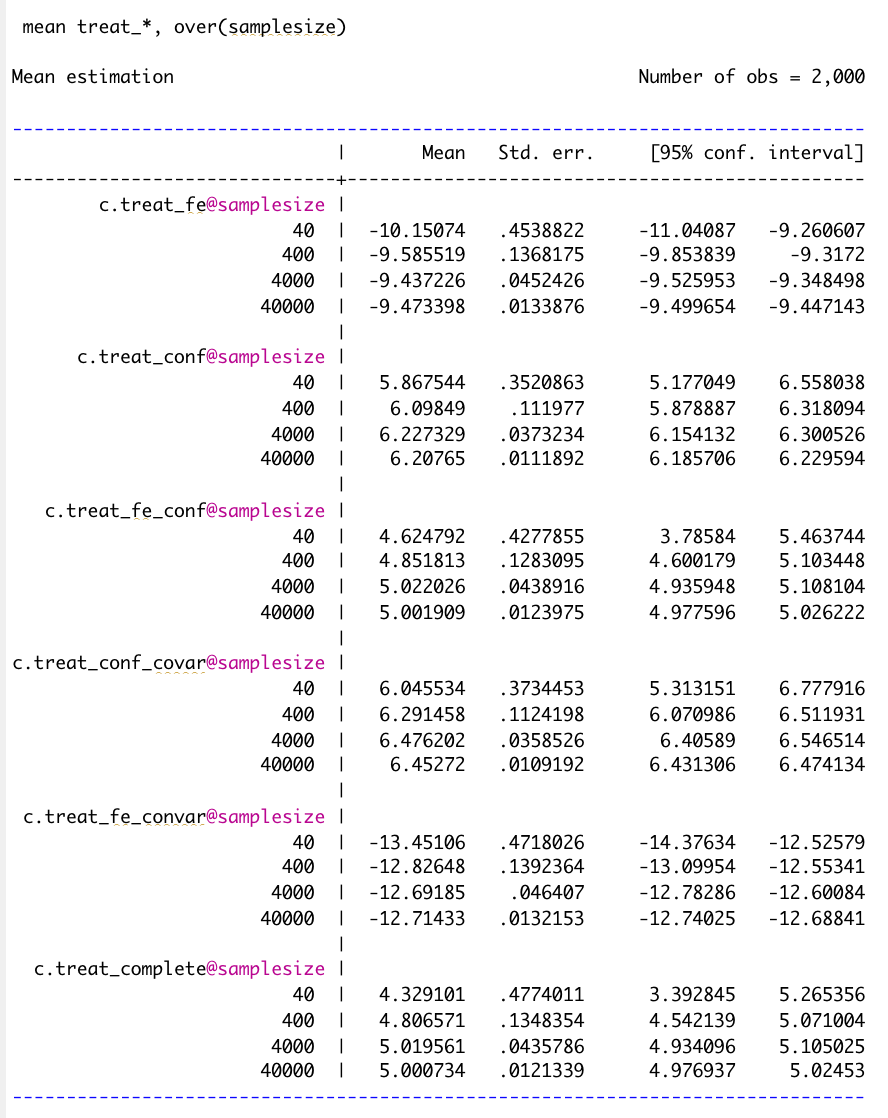
\includegraphics{img/table1.png}
\caption{Table showing mean of Betas}
\end{figure}

These findings are then ploted on a boxplot below:

\begin{figure}
\centering
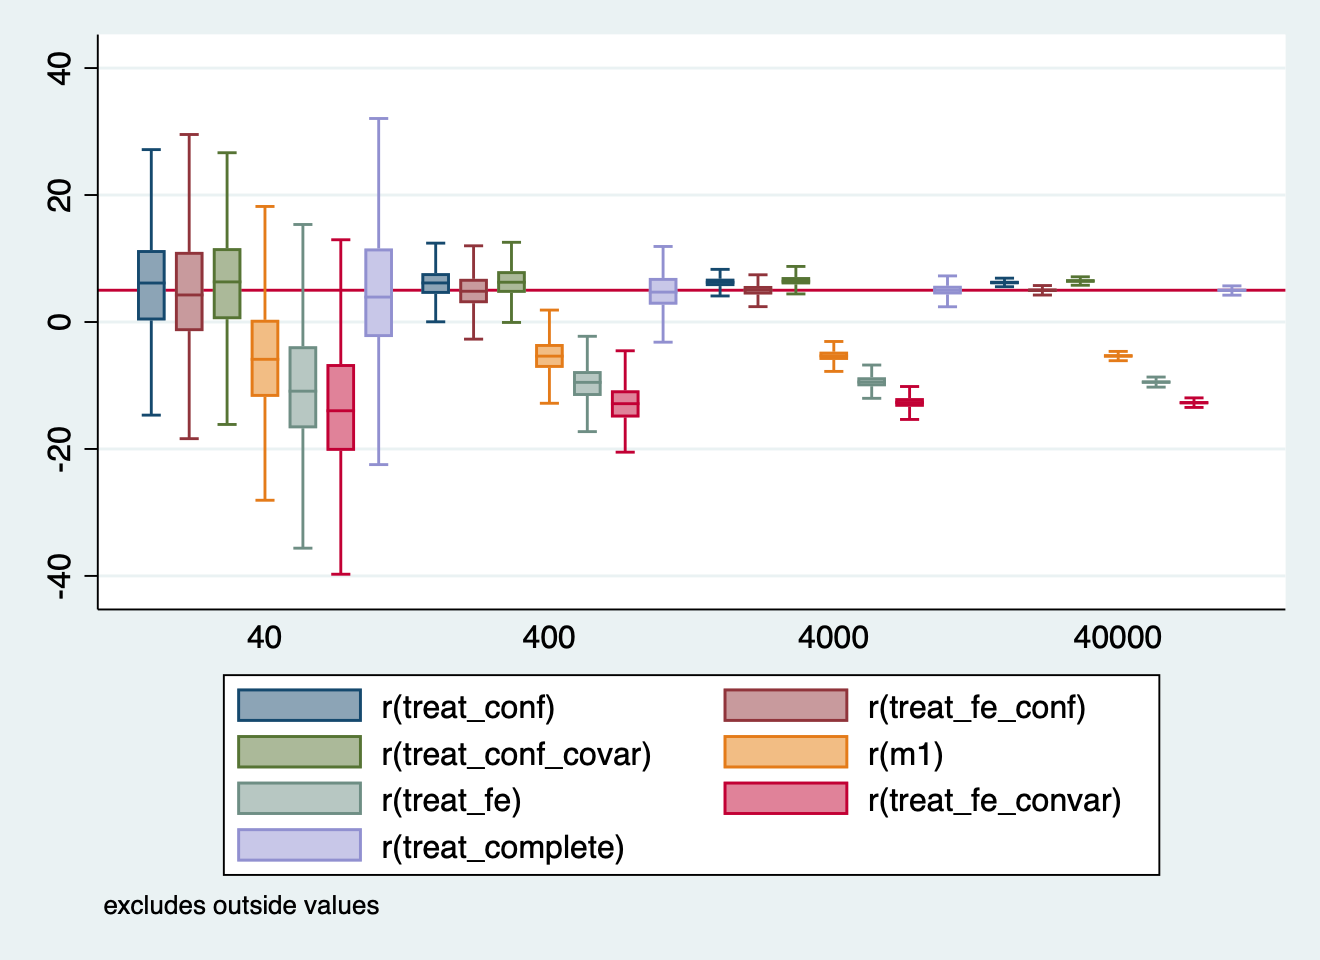
\includegraphics{img/biasbox.png}
\caption{Mean and Variance of Beta vs true parameter value}
\end{figure}

Where the x axis represents N and the Y-axis the Variance of Beta, and
where outliers have been eliminated.

And where:

m1 = reg y treatment

treat\_fe = reg y treatment i.strata

treat\_conf = reg y treatment cov\_xy

treat\_fe\_conf = reg y treatment i.strata cov\_xy

treat\_conf\_covar = reg y treatment cov\_xy cov\_x cov\_y

treat\_fe\_convar = reg y treatment i.strata cov\_x cov\_y

treat\_complete = reg y treatment i.strata cov\_xy cov\_x cov\_y

From the table we can see the c.treat\_fe and c.treat\_fe\_convar
regardless of their N are the most biased regressions as their mean is
far from the ``true'' parameter value of 5. Instead, the ones that
converge the most to the ``true'' parameter value are c.treat\_complet
and c.treat\_fe\_conf when they reach N = 40,000. We can see that as N
grows in most regression models, the means of the regressions converge
to 5, meaning the higher N the more likely to reach the ``true''
treatment effect. c.treat\_conf is the exception, but since the model
does not include covariates nor strata, it seems plausible to become
more biased as N increases.

As on the table above, we see the yellow, red, and green figures, being
the m1, c.treat\_fe and c.treat\_fe\_convar models correspondingly, are
further away from the ``true'' parameter value of 5, meaning they are
the most biased models.

Where it seems again, c.treat\_complete in purple, is the most accurate
model, the box is in the line of the ``true'' parameter, as it includes
the confounder and the covariates variables. i.e.~is the most complete
model.

Part 2:

Note again that from the model, the ``true'' parameter value is marked
at 5, because we have designed the treatment to have an effect of 5
units.

Table showing the mean and variance of beta for different regression
models, as a function of N:

\begin{figure}
\centering
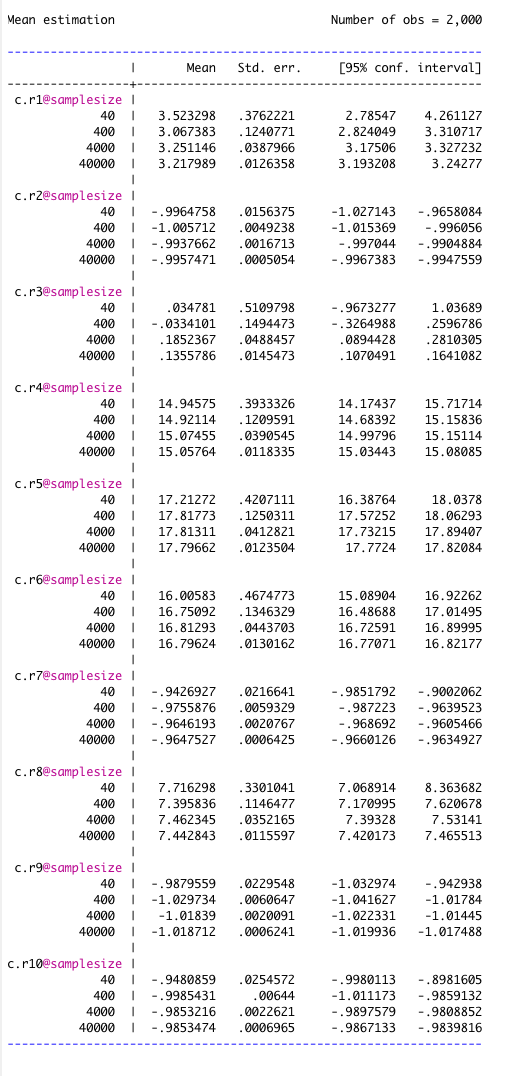
\includegraphics{img/table2.png}
\caption{Table showing mean of Betas}
\end{figure}

These findings are then ploted on a boxplot below:

\begin{figure}
\centering
\includegraphics{img/biasbox2.png}
\caption{Mean and Variance of Beta vs true parameter value for part 2}
\end{figure}

Where the x axis represents N and the Y-axis the Variance of Beta, and
where outliers have been eliminated.

where:

r1 = reg y treatment r2 = reg y treatment z coll r3 = reg y treatment z
i.strata r4 = reg y treatment z cov\_xy r5 = reg y treatment i.strata
cov\_xy r6 = reg y treatment i.strata z cov\_xy r7 = reg y treatment
i.strata z coll cov\_xy r8 = reg y treatment cov\_xy cov\_x cov\_y r9 =
reg y treatment i.strata z coll cov\_x cov\_y r10 = reg y treatment
i.strata z coll cov\_xy cov\_x cov\_y

This time none of the regression models truly converge to the ``true''
parameter, however it seems r8 is the closest. This regression includes
the confounder but not the collider nor strata. Since the purpose of the
excersise was to bias a parameter, these results match the expectation.
In Part 2, as opposed to part 1, it appears, as N grows, the regressions
become more biased, and their means move away from the true parameter.
r2 and r3 have different jumps in the means with changes in N, and this
might be caused by the fact that their models do not include neither
confounders nor covariate effects.

\end{document}
